\documentclass[aspectratio=169]{beamer}

\usepackage{amsmath, amssymb, amsxtra, amsthm, amsfonts}
\usetheme{moloch}
\usecolortheme{beaver}
\setbeamertemplate{footline}
{
  \leavevmode%
  \hbox{%
    \begin{beamercolorbox}[wd=.5\paperwidth,ht=2.25ex,dp=1ex,center]{author in head/foot}%
      \usebeamerfont{author in head/foot}\insertsection
    \end{beamercolorbox}%
    \begin{beamercolorbox}[wd=.5\paperwidth,ht=2.25ex,dp=1ex,right]{date in head/foot}%
      \usebeamerfont{date in head/foot}\inserttitle\hspace*{2em}
      \insertframenumber{} / \inserttotalframenumber\hspace*{2ex}
    \end{beamercolorbox}}%
  \vskip0pt%
}
\makeatother

\usepackage[english]{babel}
\usefonttheme{serif}

\usepackage{mathtools}
\usepackage{graphicx}
\usepackage{bm}
\usepackage{color}
\usepackage[dvipsnames,table]{xcolor}
\usepackage{tikz}
\usepackage{stanli}
\usepackage{verbatim}
\usepackage{tikz}
\usetikzlibrary{shapes,calc,through,3d,patterns}
\usetikzlibrary{decorations.pathreplacing}
\usetikzlibrary{arrows.meta,calc,positioning}

\usepackage{pgfplots}
\usepackage{siunitx} % For formatting numbers
\usepackage{hyperref}
\hypersetup{colorlinks=true,linkcolor=darkred}
\usepackage{multicol}
\usepackage[absolute,overlay,]{textpos}
\usepackage{pgfplots}
\pgfplotsset{width=10cm,compat=1.9}
\usepackage{subcaption}
\usepackage{multirow}
\usepackage{bbding}
\usepackage{arydshln}
\usepackage{mathtools}
\usepackage{tcolorbox}
\usepackage{animate}

\textblockorigin{80mm}{45mm}


\newtheorem{thm}{Theorem}
\newtheorem{cor}[thm]{Corollary}
\newtheorem{prop}[thm]{Proposition}
\newtheorem{lem}[thm]{Lemma}
\theoremstyle{remark}
\newtheorem*{rem}{Remark}

%Block def
\definecolor{darkred}{rgb}{0.6,0,0}
\setbeamertemplate{blocks}[rounded][shadow=false]
\setbeamercolor{block title}{bg=darkred!15,fg=black}
\setbeamercolor{block body}{bg=darkred!5,fg=black}

\setbeamercolor{itemize item}{fg=darkred}
\setbeamercolor{itemize subitem}{fg=darkred}
\setbeamercolor{itemize subsubitem}{fg=darkred}
\setbeamercolor{enumerate item}{fg=darkred}
\setbeamercolor{button}{bg=gray!30,fg=darkred}

\setbeamertemplate{itemize item}[square]
\setbeamertemplate{itemize subitem}[circle]
\setbeamertemplate{itemize subsubitem}[triangle]
\setbeamertemplate{enumerate items}[circle]
\setbeamercolor{item projected}{bg=darkred}

\newcommand{\bolddelta}{\boldsymbol\delta}
\newcommand{\boldxi}{\boldsymbol\xi}
\DeclareMathOperator*{\A}{\text{\raisebox{-0.2cm}{\Huge A}}}




\title{Analysis of free vibrations}
\subtitle{Analysis of free and forced vibrations}
\author{ME473 Dynamic finite element analysis of structures}
\institute{Stefano Burzio}
\date{2025}

\begin{document}
\usenavigationsymbolstemplate{}
{\setbeamertemplate{footline}{}

  \frame{\titlepage
    \begin{tikzpicture}[overlay, remember picture]
      \node[anchor=north east, xshift=-.9cm] at (current page.north east)
      {
\includegraphics[width=2cm]{../images/epfl_logo.png}};
      \node[anchor=south east, xshift=-.87cm, yshift=.05cm] at (current page.south east)  {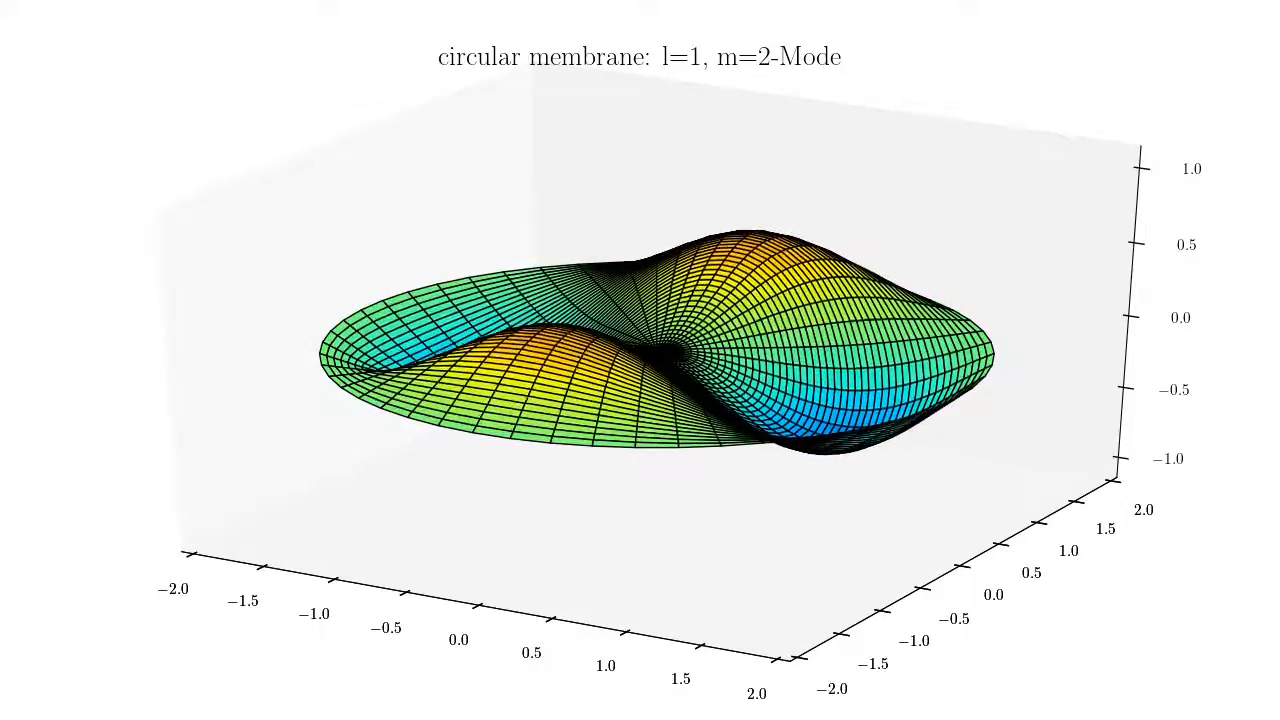
\includegraphics[height=3.7cm]{../images/eigenmodeCircularMembrane.png}};
    \end{tikzpicture}
  }

  \begin{frame}{Where do we stand?}
    \begin{center}
      \begin{tabular}{|c|l|l|l|}
        \hline
        \rowcolor{darkred!20}\textbf{Week} & \textbf{Module}                                & \textbf{Lecture topic}             & \textbf{Mini-projects} \\
        \hline

        1                                  & \multirow{6}{7em}{Linear elastodynamics}       & Strong and weak forms              &                        \\ \cline{1-1} \cline{3-4}
        2                                  &                                                & Galerkin method                    &                        \\ \cline{1-1} \cline{3-4}
        3                                  &                                                & Finite element method              & Groups formation       \\ \cline{1-1} \cline{3-4}
        4                                  &                                                & Systematization of the procedure   & Project 1 statement    \\
        \cline{1-1} \cline{3-4}
        5                                  &                                                & 3d elements, numerical integration &                        \\
        \hline
        6                                  & \multirow{5}{7em}{Special structural elements} & Bars and trusses                   &                        \\
        \cline{1-1} \cline{3-4} 7          &                                                & Planar beams                       & Project 1 submission   \\
        \cline{1-1} \cline{3-4} 8          &                                                & Frames and grids                   & Project 2 statement    \\

        \cline{1-1} \cline{3-4} 9          &                                                & Kirchhoff-Love plates              &                        \\
        \cline{1-1} \cline{3-4}
        10                                 &                                                & Reissner-Mindlin plates            &                        \\
        \cline{1-1} \cline{3-4}
        11                                 &                                                & Shells                             & Project 2 submission   \\
        \hline
        12                                 & \multirow{2}{7em}{Free and forced vibrations}  & Analysis of free vibrations        & Project 3 statement    \\
        \cline{1-1} \cline{3-4} 13         &                                                & Analysis of free vibrations        &                        \\
        \hline
      \end{tabular}
    \end{center}
    \vspace{1cm}
  \end{frame}

  \begin{frame}
    \textbf{\large Summary}
    \begin{itemize}
      \item Recap week 12
      \item Numerical modal extraction algorithms for conservative systems
      \item Rayleigh's quotient
      \item Inverse iteration algorithm
      \item Subspace algorithm
    \end{itemize}
    \vspace{.5cm}

    \textbf{\large Recommended readings}
    \begin{itemize}
      \item[(B)] Bathe, Finite Element Procedures in Engineering Analysis (chap. 10 and 11)
      \item[(P)] Petyt, Introduction to finite element vibration analysis (chap. 11)
      \item[(G)] Gmür, Dynamique des structures (§4.1 and §4.2)
      \item[(H)] Hughes, The finite element method (chap. 10)
    \end{itemize}
  \end{frame}
}

\section{Recap week 12}
 {\setbeamercolor{background canvas}{bg=darkred!5}
  \setbeamercolor{block body}{bg=darkred!5,fg=black}
  \begin{frame}{Free vibrations of non-rotating conservative systems}
    The discretization of linear three-dimensional elastodynamics, as well as the analysis of vibrations in beams and plates via FEM, all lead to a system of ODE:
    \[
      \mathbf{M} \ddot{\mathbf{q}}(t) + \mathbf{K} \mathbf{q}(t) = \mathbf{r}(t),
    \]
    \begin{columns}[T]
      \begin{column}{.4\textwidth}
        \vspace{-1cm}
        \begin{center}
          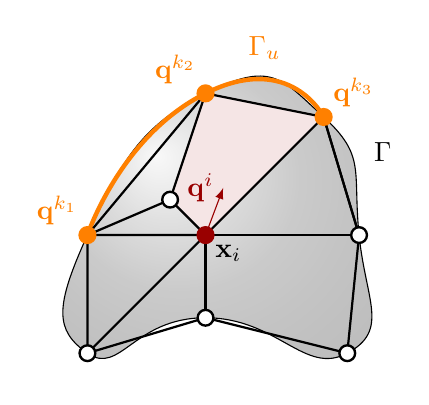
\begin{tikzpicture}[scale=1.5]
            %\draw[step=1.0,black,thin] (0,0) grid (4,4);
            % Draw the potato-like shape
            \shade [ball color= gray!90!black, opacity=.3] plot [thick,smooth cycle, tension=1] coordinates  {(1,2) (2,3.2) (3,3) (3.3,2) (3.2,1) (2,1.3) (1,1)};
            \draw[thin] plot [smooth cycle, tension=1] coordinates {(1,2) (2,3.2) (3,3) (3.3,2) (3.2,1) (2,1.3) (1,1)};
            \draw[ultra thick, orange] plot [smooth, tension=1.3] coordinates {(1,2) (2,3.2) (3,3)};
            \draw[fill=darkred!30,thick,darkred!10] (2,2) -- (3,3) -- (2,3.2) -- (1.7,2.3) -- cycle;
            \node[below right] at (2,2) {$\mathbf x_i$};
            \draw[-latex,darkred] (2,2) -- (2.15,2.4) node[darkred, left]{$\mathbf q^i$};
            % Label the boundary Gamma
            \node at (3.5,2.7) {$\Gamma$};
            \node[orange, above] at (2.5,3.4) {$\Gamma_u$};
            \draw[thick] (1,2) -- (2,3.2) -- (3,3) -- (3.3,2) -- (3.2,1) -- (2,1.3) -- (1,1) -- cycle;
            \draw[thick] (1,2) -- (2,2) -- (3,3) -- (3.3,2);
            \draw[thick] (2,1.3) -- (2,2) -- (3.3,2);
            \draw[thick] (1,1) -- (2,2) -- (1.7,2.3) -- (2,3.2);
            \draw[thick] (1.7,2.3) -- (1,2);
            \node[darkred,draw,shape=circle,fill=darkred,minimum size=2mm,line width=0.3mm,inner sep=0] at (2,2) {};
            \node[draw,shape=circle,fill=white,minimum size=2mm,line width=0.3mm,inner sep=0] at (1,1) {};
            \node[orange,draw,shape=circle,fill=orange,minimum size=2mm,line width=0.3mm,inner sep=0] at (1,2) {};
            \node[draw,shape=circle,fill=white,minimum size=2mm,line width=0.3mm,inner sep=0] at (2,1.3) {};
            \node[orange,draw,shape=circle,fill=orange,minimum size=2mm,line width=0.3mm,inner sep=0] at (2,3.2) {};
            \node[draw,shape=circle,fill=white,minimum size=2mm,line width=0.3mm,inner sep=0] at (1.7,2.3) {};
            \node[orange,draw,shape=circle,fill=orange,minimum size=2mm,line width=0.3mm,inner sep=0] at (3,3) {};
            \node[draw,shape=circle,fill=white,minimum size=2mm,line width=0.3mm,inner sep=0] at (3.2,1) {};
            \node[draw,shape=circle,fill=white,minimum size=2mm,line width=0.3mm,inner sep=0] at (3.3,2) {};
            \node[orange,above left] at (1,2) {$\mathbf q^{k_1}$};
            \node[orange,above left] at (2,3.2) {$\mathbf q^{k_2}$};
            \node[orange,above right] at (3,3) {$\mathbf q^{k_3}$};
          \end{tikzpicture}
        \end{center}
      \end{column}
      \begin{column}{.65\textwidth}
        \vspace{-0.9cm}
        \begin{block}{}
          \textbf{Free vibration:} no external forcing is applied, i.e.   $\mathbf{r}(t) = \mathbf{0}.$
        \end{block}
        \begin{itemize}
          \item Generalized nodal displacements: $$\mathbf q(t)=[\mathbf q^1(t),\dots, \mathbf q^n(t)]^T.$$
          \item \textbf{Boundary conditions:} $\mathbf q^k=\hat{\mathbf q}^k$ for all $k$ such that $\mathbf x_k\in\Gamma_u$.
          \item  \textbf{Initial conditions:} $\mathbf q(0)=\mathbf u_0$ and $\dot{\mathbf q}(0)=\mathbf v_0$
        \end{itemize}
      \end{column}
    \end{columns}
  \end{frame}

  \begin{frame}
    \begin{columns}
      \begin{column}{0.42\textwidth}
        \vspace{-0.3cm}
        \begin{center}
          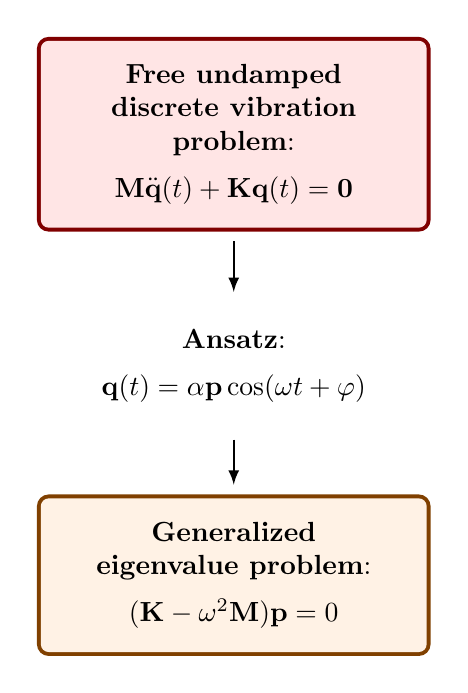
\begin{tikzpicture}[scale=0.7]
            \node (dvp) at (0,6) {
              \begin{tcolorbox}[colframe=red!50!black, colback=red!10, coltitle=black, rounded corners,width=5cm]
                \centering \textbf{Free undamped discrete vibration problem}: \\[5pt] $\mathbf{M} \ddot{\mathbf{q}}(t) + \mathbf{K} \mathbf{q}(t) = \mathbf{0}$
              \end{tcolorbox}
            };
            \node (ans) at (0,1.8) {
              \begin{tcolorbox}[colframe=white, colback=white, coltitle=black, rounded corners, width=5cm]
                \centering \textbf{Ansatz}: \\[5pt] $\mathbf q(t)=\alpha \mathbf p \cos(\omega t+\varphi)$
              \end{tcolorbox}
            };
            \node (gep) at (0,-2) {
              \begin{tcolorbox}[colframe=orange!50!black, colback=orange!10, coltitle=black, rounded corners,width=5cm]
                \centering \textbf{Generalized eigenvalue problem}: \\[5pt] $(\mathbf{K} - \omega^2 \mathbf{M}) \mathbf{p} = 0$
              \end{tcolorbox}
            };
            % Drawing arrows
            \draw[-latex, thick] (dvp.south) -- (ans.north);
            \draw[-latex, thick] (ans.south) -- (gep.north);
          \end{tikzpicture}
        \end{center}
      \end{column}
      \begin{column}{0.54\textwidth}
        \textbf{Solving the eigenvalue problem:}
        $$n=\text{dim}(\mathbf K)=\text{dim}(\mathbf M)$$
        There are $n$ eigenvalues $\lambda_j$ and $n$ corresponding eigenvectors $\mathbf p_j$ such that:
        \begin{block}{}
          \textbf{Eigenvalues} (\emph{natural frequencies} squared): $\lambda_j=\omega_j^2$ are the roots of the characteristic polynomial:
          $$\text{det}(\mathbf K-\lambda\mathbf M)=0.$$
        \end{block}
        \begin{block}{}
          \textbf{Eigenvectors} (\emph{modal shapes}): $\mathbf p_j$ are the solution of the equation
          $$(\mathbf{K} - \lambda_j \mathbf{M})\mathbf p_j=\mathbf 0.$$
        \end{block}
      \end{column}
    \end{columns}
  \end{frame}

  \begin{frame}{Rigid body modes}
    In the semi-discrete weak form obtained via finite element discretization:
    \begin{itemize}
      \item The \textbf{mass matrix} \( \mathbf{M} \) is symmetric and strictly positive definite.
      \item The \textbf{stiffness matrix} \( \mathbf{K} \) is symmetric and positive semi-definite:
            \[
              \mathbf{K} \mathbf{p} = \mathbf{0} \quad \text{for certain nonzero vectors } \mathbf{p}.
            \]
    \end{itemize}
    Consequently, the eigenvalues \( \lambda_j\) of the generalized eigenvalue problem are all real and non-negative:
    \[
      0 \,\leq\, \omega_1 \leq \omega_2 \leq \dots \leq \omega_n.
    \]

    \begin{block}{}
      \textbf{Rigid body modes:} zero eigenvalues (i.e., \( \omega_j = 0 \)) correspond to \emph{rigid body motions}, where the system undergoes displacement without internal deformation.
    \end{block}
  \end{frame}

  \begin{frame}{Orthonormalization of mode shapes}
    \begin{block}{}
      Let $\mathbf p_i$ and $\mathbf p_j$ two eigenvectors corresponding to the  eigenvalues $\lambda_i$ and $\lambda_j$, then
      $$
        \mathbf p_i^T\mathbf M\mathbf p_j  =\delta_{ij}
        \qquad\text{and}\qquad
        \mathbf p_i^T\mathbf K\mathbf p_j  =\omega_i^2\delta_{ij}
      $$
      where $\delta_{ij}$ represent Kronecker symbol.
    \end{block}
    \textbf{Consequences:} if we organize the modal vectors $\mathbf p_i$ in a so-called modal matrix $\mathbf P$:
    $$\mathbf P=\left[ \begin{array}{c;{2pt/2pt}c;{2pt/2pt}c;{2pt/2pt}c}
          \mathbf p_{1} & \mathbf p_{2} & \dots & \mathbf p_{n} \\
        \end{array}\right]$$
    then
    \begin{block}{}
      $$  \mathbf P^T\mathbf M\mathbf P  =\mathbf I       \qquad\text{and}\qquad
        \mathbf P^T\mathbf K\mathbf P  =\mathbf\Lambda$$
      where $\mathbf I$ is the identity matrix of order $n$ and $\mathbf\Lambda$ the \emph{spectral matrix}:
      $$\mathbf\Lambda=\text{diag}(\lambda_1,\dots,\lambda_n)=\text{diag}(\omega_1^2,\dots,\omega_n^2).$$
    \end{block}
  \end{frame}
 }

\section{Numerical modal extraction algorithms}

\begin{frame}{Transformation to standard form by inversion}
  \vspace{-0.5cm}
  \begin{center}
    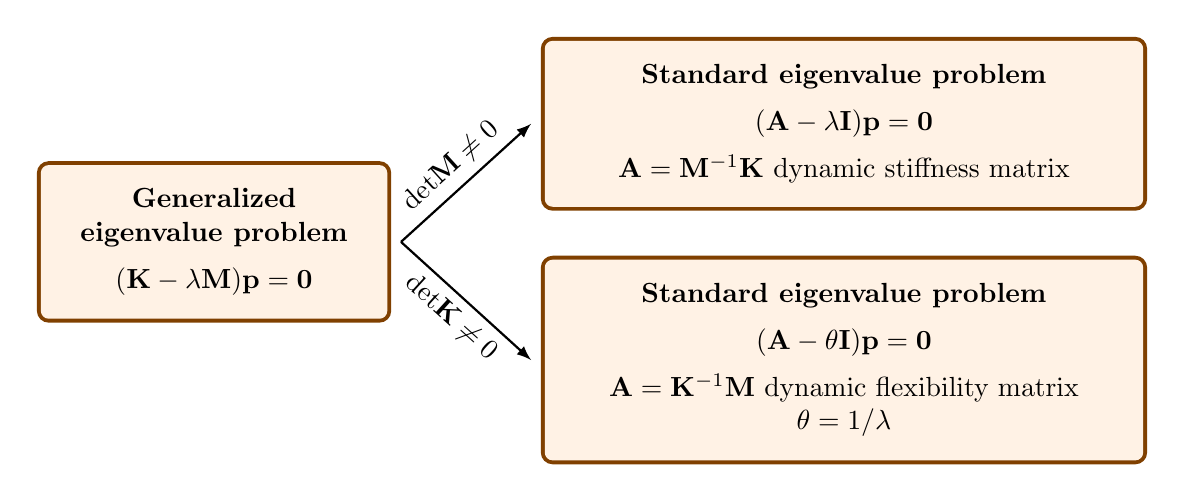
\begin{tikzpicture}
      \node (gev) at (-4,0) {
        \begin{tcolorbox}[colframe=orange!50!black, colback=orange!10, coltitle=black, rounded corners,width=4.5cm]
          \centering \textbf{Generalized eigenvalue problem} \\[5pt] $(\mathbf{K} - \lambda \mathbf{M})\mathbf p=\mathbf 0$
        \end{tcolorbox}
      };

      \node (sev1) at (4,1.5) {
        \begin{tcolorbox}[colframe=orange!50!black, colback=orange!10, coltitle=black, rounded corners,width=7.7cm]
          \centering \textbf{Standard eigenvalue problem} \\[5pt]  $(\mathbf A - \lambda \mathbf{I})\mathbf p=\mathbf 0$ \\[5pt]
          $\mathbf{A}=\mathbf{M}^{-1}\mathbf{K}$ dynamic stiffness matrix
        \end{tcolorbox}
      };

      \node (sev2) at (4,-1.5) {
        \begin{tcolorbox}[colframe=orange!50!black, colback=orange!10, coltitle=black, rounded corners,width=7.7cm]
          \centering \textbf{Standard eigenvalue problem} \\[5pt]  $(\mathbf A - \theta \mathbf{I})\mathbf p=\mathbf 0$ \\[5pt]
          $\mathbf{A}=\mathbf{K}^{-1}\mathbf{M}$ dynamic flexibility matrix \\
          $\theta=1/\lambda$
        \end{tcolorbox}
      };
      \draw[-latex, thick] (gev.east) -- (sev1.west) node[midway,sloped, above] {$\text{det}\mathbf M\neq 0$};

      \draw[-latex, thick] (gev.east) -- (sev2.west) node[midway,sloped, below] {$\text{det}\mathbf K\neq 0$};
    \end{tikzpicture}
  \end{center}
  \begin{block}{}
    \centering \textcolor{darkred}{\textbf{The matrices $\mathbf{M}^{-1}\mathbf{K}$ and  $\mathbf{K}^{-1}\mathbf{M}$ are not symmetric.}}
  \end{block}
\end{frame}

\begin{frame}{Transformation to standard form by decomposition}
  To reduce to a standard eigenvalue problem:
  \vspace{0.2cm}
  \begin{itemize}
    \item Let \( \mathbf{L} \) be the \emph{Cholesky factor} of \( \mathbf{M} \): \( \mathbf{M} = \mathbf{L} \mathbf{L}^T\).
          \begin{block}{}
            Since $\mathbf M$ is symmetric positive-definite, $\mathbf L$ is a real lower triangular matrix with positive diagonal entries.
          \end{block}
    \item Define the change of variables \( \mathbf{v} = \mathbf{L}^T \mathbf{p} \). Substituting into the original problem and multiplying by \( \mathbf{L}^{-1} \) yields:
          \[
            (\mathbf{K} - \omega^2 \mathbf{L} \mathbf{L}^T) \mathbf{p} =0
            \quad \Rightarrow \quad
            (\mathbf L^{-1}\mathbf{K}\mathbf L^{-T} - \omega^2 \mathbf{I}) \mathbf{v}=0.
          \]
    \item  Standard eigenvalue problem for symmetric and positive definite matrix \( \mathbf A=\mathbf L^{-1}\mathbf{K}\mathbf L^{-T}\):
          \[
            (\mathbf A - \lambda \mathbf{I})\mathbf v=\mathbf 0.
          \]

  \end{itemize}
  \begin{block}{}
    The eigenvalues or the standard problem are the same as those of the generalized problem, and the eigenvectors are related by \( \mathbf{p} = \mathbf{L}^{-T} \mathbf{v} \).
  \end{block}
\end{frame}

\begin{frame}{Transformation to standard form by decomposition}


  \begin{itemize}
    \item   Cholesky decomposition can be applied to $\mathbf K$ as well, since $\mathbf K$ is symmetric positive-definite:
          \[
            \mathbf{K} = \mathbf{L} \mathbf{L}^T.
          \]
    \item  Standard eigenvalue problem for symmetric and positive definite matrix \( \mathbf A=\mathbf L^{-1}\mathbf{M}\mathbf L^{-T}\):
          \[
            (\mathbf A - \theta \mathbf{I})\mathbf v=\mathbf 0.
          \]
  \end{itemize}
  \begin{block}{}
    The eigenvalues or the standard problem are related to those of the generalized problem by \( \theta = 1/\lambda \), and the eigenvectors are related by \( \mathbf{p} = \mathbf{L}^{-T} \mathbf{v} \).
  \end{block}
\end{frame}

\begin{frame}{Small and large scale problems}
  \vspace{-0.3cm}
  \begin{tcolorbox}[colback=darkred!10,colframe=darkred!40!black]
    Economical computation algorithms for extracting $(\lambda_j,\mathbf p_j)$ for $1\leq j \leq n_{modes}$ are required in practical applications, where $n_{modes}\ll n$ is the number of desired eigenpairs.
  \end{tcolorbox}

  \begin{columns}[T]
    \begin{column}{.48\textwidth}
      \textbf{Small-scale problems}
      \begin{itemize}
        \item system matrices are of modest size $n\leq 250$ or $250\leq n \leq 2500$ and small bandwidth matrices.
        \item An explicit reduction to standard eigenvalue form is typically employed:
              \begin{itemize}
                \item\emph{Generalized Jacobi method}
                \item \emph{Householder QR-algorithm}
              \end{itemize}
      \end{itemize}
    \end{column}
    \begin{column}{.48\textwidth}
      \textbf{Large-scale problems}
      \begin{itemize}
        \item $n\geq 2500$.
        \item The most effective algorithms are:
              \begin{itemize}
                \item \emph{Subspace iteration method},
                \item \emph{Lanczos' method},
                \item \emph{Irons-Guyan reduction method},
                \item \emph{Arnoldi method}
                \item \emph{Davidson method}.
              \end{itemize}
      \end{itemize}
    \end{column}
  \end{columns}
\end{frame}


\section{Rayleigh's quotient}

\begin{frame}{Definition and first properties}
  \begin{block}{}
    Let $\mathbf w$ be a vector in $\mathbb R^n$, the \textbf{Rayleigh's quotient} associated to the matrix pair $(\mathbf K,\mathbf M)$ is defined as the scalar function:
    $$\mathcal R(\mathbf w)=\frac{\mathbf w^T\mathbf K\mathbf w}{\mathbf w^T\mathbf M\mathbf w}$$
  \end{block}
  \textbf{Properties}
  \begin{enumerate}
    \item Homogeneity. Let $\alpha$ a non-zero constant, then
          $$\mathcal{R}(\alpha\mathbf w)=\frac{(\alpha\mathbf w)^T\mathbf K(\alpha\mathbf w)}{(\alpha\mathbf w)^T\mathbf M(\alpha\mathbf w)}=\frac{\alpha^2\, \mathbf w^T\mathbf K\mathbf w}{\alpha^2\, \mathbf w^T\mathbf M\mathbf w}=\mathcal{R}(\mathbf w)$$
    \item Rayleigh quotient of an eigenvector:
          $$\mathcal{R}(\mathbf w=\mathbf p_i)=\frac{\mathbf p_i^T\mathbf K\mathbf p_i}{\mathbf p_i^T\mathbf M\mathbf p_i}=\lambda_i=\omega_i^2$$
  \end{enumerate}
\end{frame}

\begin{frame}{Stationarity of Rayleigh's quotient}
  First variation of Rayleigh's quotient:
  \begin{align*}
    \delta \mathcal{R}(\mathbf{w})
     & = \frac{2(\bolddelta \mathbf{w}^T\mathbf{K} \mathbf{w})(\mathbf{w}^T\mathbf{M} \mathbf{w})
    - 2(\mathbf{w}^T\mathbf{K} \mathbf{w})(\bolddelta\mathbf{w}^T\mathbf{M} \mathbf{w})}{(\mathbf{w}^T\mathbf{M} \mathbf{w})^2}              \\[0.8em]
     & = \frac{2 \, \bolddelta \mathbf{w}^T}{\mathbf{w}^T\mathbf{M} \mathbf{w}}
    \left( \mathbf{K} \mathbf{w} - \frac{\mathbf{w}^T\mathbf{K} \mathbf{w}}{\mathbf{w}^T\mathbf{M} \mathbf{w}} \mathbf{M} \mathbf{w} \right) \\[0.8em]
     & = \frac{2 \, \bolddelta \mathbf{w}^T}{\mathbf{w}^T\mathbf{M} \mathbf{w}}
    {\color{darkred}(\mathbf{K} - \mathcal{R}(\mathbf{w}) \mathbf{M})\mathbf{w}}
  \end{align*}
  \vspace{-0.3cm}
  \begin{block}{\color{darkred} \textbf{Stationary Rayleigh's quotient in the vicinity of an modal shape !}}
    If $\mathbf{w} = \mathbf{p}_i$ then
    \[
      (\mathbf{K} - \mathcal{R}(\mathbf{w}) \mathbf{M})\mathbf{w} = (\mathbf{K} - \lambda_i \mathbf{M}) \mathbf{p}_i  = 0
    \]
  \end{block}
\end{frame}

\begin{frame}{Rayleigh principle}
  Modal expansion:
  \[
    \mathbf{w} = z_1 \mathbf{p}_1 + z_2 \mathbf{p}_2 + \cdots + z_i \mathbf{p}_i + \cdots + z_n \mathbf{p}_n = \mathbf{Pz}
  \]
  where
  \begin{align*}
    \mathbf{P} & = [\mathbf{p}_1, \mathbf{p}_2, \dots, \mathbf{p}_i, \dots, \mathbf{p}_n] \quad \text{modal matrix} \\
    \mathbf{z} & = [z_1, z_2, \dots, z_i, \dots, z_n]^T \quad \text{coefficient vector }
  \end{align*}
  Then
  \[
    \mathcal{R}(\mathbf{w} = \mathbf{Pz}) = \frac{\mathbf{z}^T \mathbf{P}^T \mathbf{K} \mathbf{Pz}}{\mathbf{z}^T \mathbf{P}^T \mathbf{M} \mathbf{Pz}} = \frac{\mathbf{z}^T \mathbf{\Lambda} \mathbf{z}}{\mathbf{z}^T \mathbf{z}} =
    \frac{\sum_{i=1}^n \lambda_i z_i^2}{\sum_{i=1}^n z_i^2}
  \]

  \bigskip
  If, without loss of generality, we impose \( \mathbf{w}^T \mathbf{M} \mathbf{w} = 1 \), then $ \mathbf{z}^T \mathbf{z} = \sum_{i=1}^n z_i^2 = 1$ and
  $$ \mathcal{R}(\mathbf{w} = \mathbf{Pz}) = \sum_{i=1}^n \lambda_i z_i^2 $$

\end{frame}

\begin{frame}{Rayleigh principle (continued)}
  Let us consider an eigenvalue \( \lambda_j \), then we can rewrite the Rayleigh's quotient as:
  \[
    \mathcal{R}(\mathbf{w}) = \sum_{i=1}^n \lambda_i z_i^2 = \lambda_j - \lambda_j + \sum_{i=1}^n \lambda_i z_i^2 = \lambda_j - \lambda_j \left( \sum_{i=1}^n z_i^2 \right) + \sum_{i=1}^n \lambda_i z_i^2
  \]
  \[
    = \lambda_j + \sum_{i=1}^n (\lambda_i - \lambda_j) z_i^2
  \]

  \bigskip

  With eigenvalues ordered as \( \lambda_1 \leq \lambda_2 \leq \cdots \leq \lambda_i \leq \cdots \leq \lambda_n \), we have:
  \begin{itemize}
    \item If \( j = 1 \), then \( \lambda_i - \lambda_1 \geq 0 \) for all \( i \), hence
          \[
            \mathcal{R}(\mathbf{w}) = \lambda_1 + \sum_{i=1}^n (\lambda_i - \lambda_1) z_i^2 \geq \lambda_1.
          \]
    \item If \( j = n \), then \( \lambda_i - \lambda_n \leq 0 \) for all \( i \), hence
          \[
            \mathcal{R}(\mathbf{w}) = \lambda_n + \sum_{i=1}^n (\lambda_i - \lambda_n) z_i^2 \leq \lambda_n.
          \]
  \end{itemize}
\end{frame}


\begin{frame}{Rayleigh quotient bounding theorem}
  \begin{tcolorbox}[colback=darkred!10,colframe=darkred!40!black]
    \begin{itemize}
      \item \textbf{Courant-Fischer formulas:}
            \[
              \mathcal{R}(\mathbf{w}) \geq \lambda_1 = \min_{\mathbf{w}} \mathcal{R}(\mathbf{w}) \]
            \[
              \mathcal{R}(\mathbf{w}) \leq \lambda_n = \max_{\mathbf{w}} \mathcal{R}(\mathbf{w})
            \]
      \item \textbf{Bounding theorem:}
            \vspace{0.2cm}
            \[
              \lambda_1 \leq \mathcal{R}(\mathbf{w}) \leq \lambda_n
            \]
    \end{itemize}
  \end{tcolorbox}
\end{frame}

\begin{frame}{Modal frequencies and shapes search via Rayleigh quotient minimization}
  \begin{enumerate}
    \item[(1)] Find $\lambda_1$ by minimization: $$\lambda_1 = \min_{\mathbf{w}}
            \mathcal{R}(\mathbf{w})$$
    \item[(2)] Find $\mathbf p_1$ by solving $(\mathbf{K} - \lambda_1 \mathbf{M}) \mathbf{p}_1  = 0$.
          \vspace{0.3cm}
    \item[(3)] Find $\lambda_2$ by minimization: $$\lambda_2 = \min_{\mathbf{w}} [\mathcal{R}(\mathbf{w}); \, \mathbf{w}^T \mathbf{M} \mathbf{p}_1 = 0]$$
    \item[(4)] Find $\mathbf p_2$ by solving $(\mathbf{K} - \lambda_2 \mathbf{M}) \mathbf{p}_2  = 0$.
          \[
            \vdots
          \]
    \item[(j)]  Find $\lambda_j$ by minimization: $$\lambda_j = \min_{\mathbf{w}} [\mathcal{R}(\mathbf{w}); \, \mathbf{w}^T \mathbf{M} \mathbf{p}_i = 0, \, i = 1, 2, \dots, j-1]$$
    \item[(j+1)] Find $\mathbf p_j$ by solving $(\mathbf{K} - \lambda_j \mathbf{M}) \mathbf{p}_j  = 0$.
  \end{enumerate}
\end{frame}

\section{Example: Longitudinal vibrations of a free-free bar}

\begin{frame}{Rayleigh quotient for longitudinal vibrations of free-free bar}
  Consider a free-free bar discretized by one bilinear element.
  \begin{columns}
    \column{0.65\textwidth}
    \begin{center}
      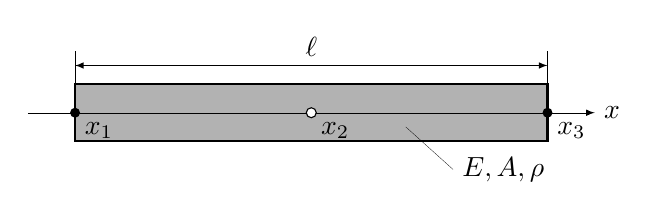
\begin{tikzpicture}[scale=0.6]
        % Draw the rectangle
        \filldraw[fill=gray!60, draw=black,thick] (0,-0.6) rectangle (10,0.6);
        %axis
        \draw[-latex, ultra thin] (-1,0) -- (11,0) node[right]{$x$};
        % length
        \draw[ultra thin] (10,0) -- (10, 1.3) ;
        \draw[ultra thin] (0,0) -- (0,1.3);
        \draw[latex-latex, ultra thin]  (0,1)  to node[sloped,midway,above] {$\ell$}(10,1) ;
        \draw[ultra thin]  (7,-0.3) -- (8,-1.2) node[right]{$E,A,\rho$};

        \fill (0,0) circle (3pt) node[below right] {$x_1$};
        \fill (10,0) circle (3pt) node[below right] {$x_3$};
        \draw[fill=white, draw=black] (5,0) circle (3pt) node[below right] {$x_2$};
      \end{tikzpicture}
    \end{center}
    \column{0.5\textwidth}
    {\small \begin{itemize}
        \item $\ell$ length
        \item $A$ cross-sectional area
        \item $E$ Young's modulus
        \item $\rho$ material density
      \end{itemize}}
  \end{columns}
  \begin{block}{}
    \textbf{Objective}:\newline\noindent
    Compute the approximated natural frequencies and corresponding mode shapes via the minimization of Rayleigh's quotient
  \end{block}
\end{frame}

\begin{frame}{MATLAB example - longitudinal vibrations of free-free bar}
  \begin{center}
    \href{https://drive.mathworks.com/sharing/6a9792ef-d0a7-4aca-a1d0-8b1862b0ac3b}{\beamergotobutton{Go to Matlab Drive}}
  \end{center}
\end{frame}

\section{Rayleigh-Ritz analysis}

\begin{frame}{Rayleigh-Ritz analysis: fundamentals}
  \begin{block}{}
    \textbf{Goal:} approximate the lowest $n_{modes}$ eigenvalues and corresponding eigenvectors of the generalized eigenproblem \( \mathbf K\mathbf p = \lambda\mathbf M \mathbf p \)
  \end{block}

  \textbf{Inputs:}
  \begin{itemize}
    \item \(\mathbf K \), \(\mathbf M \): positive definite stiffness and mass matrices (or shifted to be so). If $\mathbf K$ is singular, use shift: set \( \mathbf K_\sigma =\mathbf K + \sigma\mathbf M \) with \( \sigma > 0 \).
    \item $n_{modes}$ linearly independent \textbf{Ritz basis vectors} $\boldsymbol{\psi}_i$, spanning a subspace $\mathcal S$.
  \end{itemize}

  \textbf{Output:}
  \begin{itemize}
    \item Approximated modal matrix of size $n\times n_{modes}$
          $$\mathbf P=[\mathbf p_1,\dots,\mathbf p_{n_{modes}}]$$
    \item Approximated spectral matrix: $$\mathbf \Lambda=\text{diag}(\lambda_1,\dots,\lambda_{n_{modes}})$$
  \end{itemize}
\end{frame}


\begin{frame}{Rayleigh-Ritz reduction algorithm}
  \begin{enumerate}
    \item Any trial vector in $\mathcal S$ is written as
          \(
          \mathbf w = \sum_{i=1}^{n_{modes}} x_i \boldsymbol{\psi}_i ,
          \)
          with coordinates $x_i$.
    \item Insert $\mathbf w = \mathbf \Psi \mathbf x$ into $\mathcal R(\mathbf w)$ to obtain the projected stiffness and mass matrices into the Ritz basis:
          \[
            \tilde{\mathbf K} = \mathbf \Psi^T \mathbf K \mathbf \Psi, \qquad \tilde{\mathbf M} = \mathbf \Psi^T \mathbf M \mathbf \Psi,
          \]
          where $\mathbf \Psi = [\boldsymbol{\psi}_1, \boldsymbol{\psi}_2, \dots, \boldsymbol{\psi}_{n_{modes}}]$.
    \item Solve the reduced $(n_{modes}\times n_{modes})$ generalized eigenvalue problem by minimization:
          \[
            \tilde{\mathbf K} \mathbf x = \phi\, \tilde{\mathbf M} \mathbf x .
          \]
          to obtain approximate eigenpairs $(\phi_i, \mathbf x_i)$   for \( i = 1, 2, \dots, n_{modes} \).
    \item Compute the modal and the spectral matrices:
          \[
            \tilde{\mathbf \Lambda} = \text{diag}(\phi_1, \phi_2, \dots, \phi_{n_{modes}}) ,
          \]
          and the approximate mode shapes
          \[
            \mathbf p_i = \mathbf \Psi \mathbf x_i .
          \]
  \end{enumerate}
\end{frame}

\begin{frame}{Practical aspects and remarks}
  \begin{tcolorbox}[colback=darkred!10,colframe=darkred!40!black]
    \textbf{Upper-bound property}:
    \[
      \lambda_i \le \phi_i , \qquad i=1,\dots,n_{modes} .
    \]
  \end{tcolorbox}
  \begin{itemize}
    \item Ritz basis often obtained from static solutions:
          \[
            \mathbf K \mathbf \mathbf \Psi = \mathbf R,
          \]
          where $\mathbf R$ contains chosen load patterns.
    \item Accuracy depends on how well $\mathcal S$ approximates the
          subspace of the lowest eigenmodes.
    \item Many well-known methods are special cases of Rayleigh--Ritz:
          \begin{itemize}
            \item \textbf{Static condensation} (Irons-Guyan reduction)
            \item \textbf{Component mode synthesis}
            \item \textbf{Subspace iteration}
          \end{itemize}
  \end{itemize}
\end{frame}


\section{Inverse iteration algorithm}

\begin{frame}{General idea of inverse and forward iteration}
  \vspace{-0.2cm}
  \small
  \begin{block}{}
    \textbf{Goal:} compute \textbf{one} eigenvector of the generalized eigenproblem \( \mathbf K\mathbf p = \lambda\mathbf M \mathbf p \).
  \end{block}
  \textbf{Idea:} Use an \emph{iterative} improvement of an assumed eigenvector.
  \begin{itemize}
    \item Start from an arbitrary vector $\mathbf p^{(0)}$.
    \item Generate a sequence of vectors $\mathbf p^{(1)}, \mathbf p^{(2)}, \dots$ that converge to an eigenvector.
    \item  Compute an approximate eigenvalue using Rayleigh's quotient:
          \[
            \lambda^{(k)} = \mathcal R(\mathbf p^{(k)}).
          \]
  \end{itemize}
  \begin{columns}[T]
    \begin{column}{0.5\textwidth}
      \textbf{Inverse iteration:}
      \begin{itemize}
        \item Form a \emph{“force”} vector:
              \(
              \mathbf R_1 = \mathbf M \mathbf p^{(0)}.
              \)
        \item Solve the static-like equilibrium problem:
              \[
                \mathbf K \mathbf p^{(1)} = \mathbf R_1,
              \]
        \item Repeat until convergence is met.
      \end{itemize}
    \end{column}
    \begin{column}{0.5\textwidth}
      \textbf{Forward iteration:}
      \begin{itemize}
        \item Compute $\mathbf R_1 = \mathbf K \mathbf p^{(0)}$.
        \item Solve
              \[
                \mathbf M \mathbf p^{(1)} = \mathbf R_1 ,
              \]
        \item Repeat until convergence is met.
      \end{itemize}
    \end{column}
  \end{columns}
\end{frame}


\begin{frame}{Inverse iteration algorithm}
  \small
  \textbf{Inputs:}
  \vspace{-0.3cm}
  \begin{multicols}{2}
    \begin{itemize}
      \item \(\mathbf K \), \(\mathbf M \): stiffness and mass matrices
      \item \( \mathbf p^{(0)} \): initial guess vector (non-zero)
      \item \( \sigma \): spectral shift
      \item \( \varepsilon \): convergence tolerance
    \end{itemize}
  \end{multicols}
  \vspace{-0.3cm}

  \textbf{Algorithm:}
  \begin{enumerate}
    \item If $\mathbf K$ is singular, use shift: set \( \mathbf K_\sigma =\mathbf K + \sigma\mathbf M \)
    \item For \( k = 1, 2, \dots \) until convergence:
          \begin{itemize}
            \item Solve for $\bar{\mathbf p}^{(k)}$ the static equilibrium problem  $$\mathbf K_\sigma \, \bar{\mathbf p}^{(k)} =\mathbf M \, \mathbf p^{(k-1)} $$
            \item $\mathbf M$-normalize the vector $\bar{\mathbf p}^{(k)}$:
                  $$\mathbf p^{(k)} = \bar{\mathbf p}^{(k)} / \sqrt{(\bar{\mathbf p}^{(k)})^T \mathbf M \bar{\mathbf p}^{(k)}}$$
            \item Check convergence: \( \|\mathbf p^{(k)} - \mathbf p^{(k-1)}\| < \varepsilon \)
          \end{itemize}
  \end{enumerate}
  \textbf{Output:} approximated eigenvector \( \mathbf p^{(k)} \) and eigenvalue \( \lambda^{(k)} = \mathcal R(\mathbf p^{(k)}) \).
\end{frame}

\begin{frame}{Convergence of inverse iteration}
  \begin{tcolorbox}[colback=darkred!10,colframe=darkred!40!black]
    \begin{itemize}
      \item  The inverse iteration converges to $\mathbf p_j$, the eigenvector associated with the eigenvalue closest to \( \sigma \), if the initial guess $\mathbf p^{(0)}$ is not $\mathbf M$-orthogonal to $\mathbf p_j$.
      \item     If no shift is used, i.e. $\sigma=0$, the method converges to the eigenvector associated with the \emph{smallest eigenvalue} provided the orthogonality condition on the initial guess is met.
    \end{itemize}
  \end{tcolorbox}
  \begin{itemize}
    \item The rate of convergence depends on the ratio
          \[
            \rho = \frac{|\lambda_j - \sigma|}{|\lambda_{j+1} - \sigma|},
          \]
          where \( \lambda_j \) is the eigenvalue closest to \( \sigma \) and \( \lambda_{j+1} \) is the next closest eigenvalue.
    \item If $\varepsilon=10^{-2s}$ , then approximately \( 2s \) correct digits of the eigenvector are obtained and \( s \) correct digits of the eigenvalue.
  \end{itemize}
\end{frame}

\section{Subspace iteration method}

\begin{frame}{General ideas behind the subspace iteration method}
  \vspace{-0.2cm}
  \begin{block}{}
    \textbf{Goal:} compute the lowest \( n_{modes} \ll n \) eigenpairs \( (\mathbf p_i, \lambda_i) \) of the generalized eigenproblem
    $$\mathbf K\mathbf p = \lambda\mathbf M \mathbf p.$$
  \end{block}
  Method developed and named by K. J. Bathe consists of the following three steps:
  \begin{enumerate}
    \item Establish $q$ starting iteration vectors, $q> n_{modes}$ , where $n_{modes}$ is the number of eigenvalues and vectors to be calculated.
    \item Use \textbf{inverse iteration} on the $q$ vectors and \textbf{Rayleigh-Ritz analysis} to extract the "\emph{best}" eigenvalue and eigenvector approximations from the $q$ iteration vectors.
    \item After iteration convergence, use the \textbf{Sturm sequence} check to verify that the required eigenvalues and corresponding eigenvectors have been calculated.
  \end{enumerate}
\end{frame}

\begin{frame}{Preliminary considerations}
  Named the subspace iteration method because the iteration is equivalent to iterating with a $q$-dimensional subspace $\mathcal S_k=\text{span}(\mathbf p^{(k)}_1, \dots, \mathbf p^{(k)}_q)$ and should not be regarded as a simultaneous iteration with $q$ individual iteration vectors.
  \begin{center}
    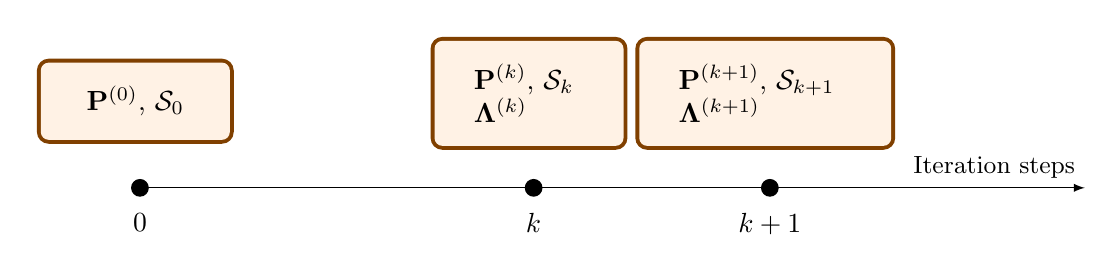
\begin{tikzpicture}
      \draw[-latex] (0,0) -- (12,0) node[above left] {\small Iteration steps};
      \filldraw (0,0) circle (3pt); % Marker
      \filldraw (5,0) circle (3pt); % Marker
      \filldraw (8,0) circle (3pt); % Marker
      \node[align=center] at (0,1.1) {
        \begin{tcolorbox}[colframe=orange!50!black, colback=orange!10, coltitle=black, rounded corners,width=2.5cm]
          \centering $\mathbf P^{(0)}$, $\mathcal S_0$
        \end{tcolorbox}
      };
      \node[align=center,below] at (0,-0.2) {$0$};
      \node[align=center] at (5,1.2) {\begin{tcolorbox}[colframe=orange!50!black, colback=orange!10, coltitle=black, rounded corners,width=2.5cm]
          $\mathbf P^{(k)}$, $\mathcal S_{k}$ \\  $\mathbf \Lambda^{(k)}$
        \end{tcolorbox}
      };
      \node[align=center, below] at (5,-0.2) {$k$};
      \node[align=center] at (8,1.2) {\begin{tcolorbox}[colframe=orange!50!black, colback=orange!10, coltitle=black, rounded corners,width=3.3cm]
          $\mathbf P^{(k+1)}$, $\mathcal S_{k+1}$ \\  $\mathbf \Lambda^{(k+1)}$
        \end{tcolorbox}
      };
      \node[align=center,below] at (8,-0.2) {$k+1$};
    \end{tikzpicture}
  \end{center}
  The effectiveness of the algorithm lies in that it is much easier to establish a $q$-dimensional starting subspace which is close to $\text{span}(\mathbf p_1, \dots, \mathbf p_{n_{modes}})$ than to find $n_{modes}$ vectors that are each close to a required eigenvector $\mathbf p_i$.
\end{frame}

\begin{frame}{Preliminary considerations}
  \begin{itemize}
    \item  All characteristics of the Ritz analysis pertain also to the subspace iteration; i.e., the smallest eigenvalues are approximated best in the iteration, and all eigenvalue approximations are \textbf{upper bounds} on the actual eigenvalues sought.
    \item Because the iteration is performed on a subspace, \textbf{convergence of the subspace} is all that is required and not convergence of individual iteration vectors to eigenvectors.
    \item If the initial vectors are linear combinations of the required eigenvectors, the solution algorithm converges in one step.
  \end{itemize}
\end{frame}

\begin{frame}{Pseudo-code of the subspace iteration method}
  \textbf{Inputs:}
  \begin{itemize}
    \item \(\mathbf K \), \(\mathbf M \): stiffness and mass matrices of dimension \( n \times n \).
    \item \( n_{modes} \): number of desired eigenmodes.
    \item \( q \): number of iteration vectors, with \( q > n_{modes} \).
    \item \(\mathbf P^{(0)} \in \mathbb{R}^{n \times q} \): initial guess matrix of linearly independent vectors
          $$\mathbf  P^{(0)}=[\mathbf p^{(0)}_1,\dots,\mathbf p^{(0)}_q]$$
    \item \( \sigma \): spectral shift (optional)
    \item \( \varepsilon \): convergence tolerance
  \end{itemize}

  \textbf{Output:}
  \begin{itemize}
    \item  Approximated eigenvectors: $\mathbf  P^{(k)}=[\mathbf p^{(k)}_1,\dots,\mathbf p^{(k)}_q]$
    \item Approximated eigenvalues: $\mathbf \Lambda^{(k)}=\text{diag}(\lambda^{(k)}_1,\dots,\lambda^{(k)}_q)$
  \end{itemize}
\end{frame}

\begin{frame}{Pseudo-code of the subspace iteration method}
  \textbf{Algorithm:}
  \begin{enumerate}
    \item If $\mathbf K$ is singular, use shift: set \( \mathbf K_\sigma =\mathbf K + \sigma\mathbf M \)
    \item For \( k = 1, 2, \dots \) until convergence:
          \begin{itemize}
            \item Do step 1: perform inverse iteration on \( q \) vectors to obtain
                  $$\overline{\mathbf P^{(k)}}.$$
            \item Do step 2a: compute the projected stiffness and mass matrices:
                  $$\mathbf K^{(k)} \qquad\text{and}\qquad \mathbf M^{(k)}.$$
            \item Do step 2b: solve the projected generalized eigenvalue problem to obtain the projected modal matrix and the spectral matrix:
                  $$\mathbf Z^{(k)} \qquad\text{and}\qquad \mathbf \Lambda^{(k)}.$$

            \item Do step 2c: calculate the updated modal matrix \( \mathbf P^{(k)} \).
            \item Do step 3: check convergence
          \end{itemize}
  \end{enumerate}
\end{frame}


\begin{frame}{Subspace iteration steps}
  \begin{enumerate}
    \item \textbf{Step 1:} Inverse iteration on \( q \) vectors: find the $(n\times q)$ matrix $\overline{\mathbf P^{(k)}}$ such that
          \[
            \mathbf K\overline{\mathbf P^{(k)}} = \mathbf M\mathbf P^{(k-1)}
          \]
    \item \textbf{Step 2a:} Compute projected stiffness and mass matrices (\(q\times q\)):
          \[
            \mathbf K^{(k)} = (\overline{\mathbf P^{(k)}})^T \mathbf K \overline{\mathbf P^{(k)}}, \quad \mathbf M^{(k)} = (\overline{\mathbf P^{(k)}})^T \mathbf M \overline{\mathbf P^{(k)}}
          \]
    \item \textbf{Step 2b:} Solve $(q\times q)$ generalized eigenvalue problem: Find the projected modal matrix $\mathbf Z^{(k)}$ and the spectral matrix $\mathbf \Lambda^{(k)}$ such that
          \[
            \mathbf K^{(k)}\mathbf Z^{(k)} = \mathbf M^{(k)}\mathbf Z^{(k)} \mathbf \Lambda^{(k)}
          \]
    \item \textbf{Step 2c:} Calculate the updated modal matrix (\(n\times q\)):
          \[
            \mathbf P^{(k)} = \overline{\mathbf P^{(k)}} \mathbf Z^{(k)}
          \]
  \end{enumerate}
\end{frame}

\begin{frame}{Step 1 - Inverse iteration on \( q \) vectors}
  Suppose that the Step 1 is replace by a simultaneous inverse iteration on \( m \) eigenvectors:
  \[
    \mathbf P^{(k)} = (\mathbf K^{-1}\mathbf M)\mathbf P^{(k-1)}=\dots = (\mathbf K^{-1}\mathbf M)^k\, \mathbf P^{(0)}
  \]
  \vspace{-0.5cm}
  \begin{block}{}
    Define the subspace \( \mathcal S^{(k)} \) of rank \( q \), spanned by the vectors \( \{\mathbf p_i^{(k)}\} \).  $\mathbf  P^{(k)}=[\mathbf p^{(k)}_1,\dots,\mathbf p^{(k)}_q]$ forms a \emph{non-orthogonal} basis of \( \mathcal S^{(k)} \).
  \end{block}
  \begin{itemize}
    \item[\XSolidBrush] All columns of \(\mathbf  P^{(k)} \) tend toward \( \mathbf  p_1 \)
    \item[\XSolidBrush]  Collinearity if no orthogonalization is applied !
  \end{itemize}

  \begin{tcolorbox}[colback=darkred!10,colframe=darkred!40!black]
    \begin{center}
      \textbf{Orthogonalization} of vectors \(\mathbf p_i^{(k)} \) at each iteration needed !
    \end{center}
  \end{tcolorbox}
\end{frame}

\begin{frame}{Modified Step 2 - Gram-Schmidt orthogonalization}
  \begin{enumerate}
    \item \textbf{Step 1:} Inverse iteration on \( q \) vectors: find the $(n\times q)$ matrix $\overline{\mathbf P^{(k)}}$ such that
          \[
            \mathbf K\overline{\mathbf P^{(k)}} = \mathbf M\mathbf P^{(k-1)}
          \]
    \item \textbf{Step 2:} Grand-Schmidt orthogonalization:
          $$\mathbf P^{(k+1)}=\mathbf P^{(k)}\mathbf R^{k}$$
          where $\mathbf R^{k}$ is an upper triangular matrix chosen in such way that
          $$(\mathbf P^{(k+1)})^T\mathbf M \mathbf P^{(k+1)} = \mathbf I$$
  \end{enumerate}
  \begin{block}{}
    Gram-Schmidt method is inefficient as iteration vector $\mathbf p_i^{(k)}$ is forced to converge to a prescribed eigenvector $\mathbf p_i$ without allowing a more effective linear combination of the iteration vectors to take place.
  \end{block}
\end{frame}

\begin{frame}{Step 2 - Orthogonalization by minimization of the Rayleigh quotient}
  \begin{itemize}
    \item Orthogonalization by minimization of the Rayleigh quotient:
          \[
            \mathcal R(\mathbf w^{(k)}) = \frac{(\mathbf w^{(k)})^T\mathbf  K \mathbf w^{(k)}}{(\mathbf w^{(k)})^T\mathbf  M\mathbf  w^{(k)}}
          \]
    \item Let \(\mathbf  w^{(k)} = \overline{\mathbf P^{(k)}}\mathbf z^{(k)} \)
    \item Projected Rayleigh's quotient:
          \[
            \mathcal R(\mathbf w^{(k)}) = \frac{(\mathbf z^{(k)})^T\mathbf K^{(k)} \mathbf z^{(k)}}{(\mathbf z^{(k)})^T\mathbf M^{(k)}\mathbf z^{(k)}}
          \]
          where
          \[
            \mathbf K^{(k)} = (\overline{\mathbf P^{(k)}})^T \mathbf K \overline{\mathbf P^{(k)}}, \quad\mathbf M^{(k)} = (\overline{\mathbf P^{(k)}})^T\mathbf M \overline{\mathbf P^{(k)}}
          \]
  \end{itemize}
\end{frame}

\begin{frame}{Step 2b - Solve projected generalized eigenvalue problem}
  \begin{itemize}
    \item Minimization of the projected Rayleigh's quotient (generalized eigenvalue problem of dimension \( q \times q \))
    \item Stationary condition:
          \[
            \delta \mathcal R(\mathbf w^{(k)}) = 0\qquad \Rightarrow\qquad \mathbf K^{(k)} \mathbf z^{(k)} = \lambda^{(k)}\mathbf  M^{(k)}\mathbf  z^{(k)}
          \]

    \item Solve via transformation method (e.g., Jacobi method):
          \[
            \mathbf K^{(k)} \mathbf Z^{(k)} =\mathbf  M^{(k)}\mathbf  Z^{(k)} \mathbf \Lambda^{(k)}
          \]
    \item Ritz vectors and values:
          \[
            \mathbf Z^{(k)} = [\mathbf z_1^{(k)}, \dots,\mathbf  z_q^{(k)}], \quad\text{and}\quad
            \mathbf \Lambda^{(k)} = \text{diag}(\mathbf \lambda_1^{(k)}, \dots, \mathbf \lambda_q^{(k)})
          \]
  \end{itemize}
\end{frame}

\begin{frame}{}
  \textbf{Step 2c - Update modal matrix and orthogonality check}
  \vspace{0.3cm}
  \begin{itemize}
    \item Update the modal matrix:
          $$\mathbf P^{(k)} = \overline{\mathbf P^{(k)}} \mathbf Z^{(k)}$$
    \item Orthogonality check:
          \[
            (\mathbf P^{(k)})^T\mathbf M\mathbf P^{(k)} =\mathbf I
          \]
  \end{itemize}

  \textbf{Step 3 - Convergence to stop iteration}\newline
  Convergence criterion based on relative change of eigenvalues:
  \[
    \frac{|\lambda_i^{(k)} - \lambda_i^{(k-1)}|}{\lambda_i^{(k)}} < \varepsilon, \quad i = 1, 2, \dots, n_{modes}
  \]
\end{frame}


\begin{frame}{Starting iteration vectors $\mathbf P^{(0)}$}
  \begin{itemize}
    \item The starting iteration vectors in $\mathbf P^{(0)}$ should not be too close to each other, i.e., they should be linearly independent.
    \item Higher convergence rate can be obtained by increasing $q$. However, using more iteration vectors will also increase the computer effort for one iteration. In practice
          $$q=\min(2n_{modes},\, n_{modes} + 8)$$
  \end{itemize}
  \begin{tcolorbox}[colback=darkred!10,colframe=darkred!40!black]
    \textbf{Empirical guidelines}
    \begin{itemize}
      \item The first column of $\mathbf P^{(0)}$ should be the diagonal of $\mathbf M$. This ensures that all mass degrees of freedom are excited.
      \item The other columns in $\mathbf P^{(0)}$, except for the last column, should be unit vectors $\mathbf e_i$, with entries $+1$ at the degrees of freedom with the smallest ratios $k_{ii}/m_{ii}$, and the last column in $\mathbf P^{(0)}$ should be a random vector with values in $[0,1]$.
    \end{itemize}
  \end{tcolorbox}
\end{frame}

\begin{frame}{Convergence of the subspace iteration method}
  \begin{itemize}
    \item Iteration is performed with $q$ vectors, $q > n_{modes}$, but convergence is measured only on the approximations obtained for the $n_{modes}$ smallest eigenvalues.
    \item If the starting iteration vectors in $\mathbf P^{(0)}$, are not orthogonal to any one of the required eigenvectors $\mathbf p_1,\dots, \mathbf p_{n_{modes}}$, then as $k\to \infty$
          $$\tilde{\mathcal S}_k=\text{span}(\mathbf p^{(k)}_1, \dots, \mathbf p^{(k)}_{n_{modes}})\to \mathcal S_\infty = \text{span}(\mathbf p_1, \dots, \mathbf p_{n_{modes}})$$\
    \item  Assuming that in the iteration
          the vectors in $\mathbf P^{(k+1)}$ are ordered in such way that the $i$-th diagonal element in $\mathbf \Lambda^{(k+1)}$ is larger
          than the $(i - 1)$-st element for $i = 2,\dots, p$, then the $i$-th column in $\mathbf P^{(k+1)}$ converges to $\mathbf p_i$ and the convergence rate is
          $$\lambda_i/\lambda_{p+1}$$
          Although this is an asymptotic convergence rate, it indicates that the smallest eigenvalues converge fastest.
  \end{itemize}
\end{frame}

\begin{frame}{Final Sturm sequence check}
  \begin{block}{}
    After convergence is achieved, a final check based on the Sturm sequence property can be performed to ensure that the number of computed eigenvalues below a certain value is correct.
  \end{block}

  \begin{itemize}
    \item The Sturm sequence property states that the number of eigenvalues of the generalized eigenvalue problem \( \mathbf K\mathbf p = \lambda\mathbf M \mathbf p \) that are less than a given value \( \lambda^* \) is equal to the number of negative pivots obtained when performing an \( \mathbf L\mathbf  D\mathbf  L^T \) factorization of the matrix \( \mathbf K - \lambda^* \mathbf M \).
    \item This property can be used to verify that the number of computed eigenvalues below a certain threshold matches the expected count, providing an additional layer of validation for the results obtained from the subspace iteration method.
  \end{itemize}
\end{frame}

\end{document}